\documentclass[titlepage, 10pt]{article}

\usepackage{graphicx} %[pdftex]
\usepackage[hidelinks]{hyperref}
\usepackage{titlepic}
\usepackage{fullpage}

\titlepic{
\includegraphics[width=0.30\textwidth]{img/sedes.jpg}}
\title
{
	[H03I7A] Design in Medical Technology\\
	Shape-based feature analysis\\
	for nodule detection in lung images
}
\author{Kim Nuyts \and Sven Van Hove}
\date{\today}

\begin{document}

\pagenumbering{roman} %i, ii, iii
\maketitle

\clearpage
\pagenumbering{Roman} %I, II, III
\tableofcontents
\clearpage

% paragraph makeup, after ToC
\setlength{\parindent}{0pt} %don't indent new paragraph
\setlength{\parskip}{2ex} %add blank line in between
\pagenumbering{arabic} %1, 2, 3

\section{Summary} %1 page

\subsection{Subsection}

\subsubsection{Subsubsection}
Text.

\subsection{Another subtitle}

More text. \cite{ginneken} \cite{abc}
\clearpage

\section{Introduction}


\section{Literature review}
\subsection{Introduction}
In order to establish a well thought pulmonary lung CAD system, the appearance
of lung abnormalities is discussed and a delineation of the term 'nodule' is
provided. Then an overview of commercial and research-based CAD systems is given
and a comparison of performances is discussed.

\subsection{The biology of lung nodules}
Pulmonary odules are lung tissue abnormalities that are roughly spherical with a
diameter up to 30 mm. On chest CT scans they appear as a rounded or irregular
opacity (\autoref{fig:nodules}). Many types of lung nodules can by distinguished
on CT scans. A centrilobular nodule is separated by several millimeters from the
pleural surfaces, fissures and interlobular septa. Micronodules are very small
nodules and have a diameter less than 3 millimeters. A ground-glass nodule -- or
non-solid nodule -- appears on the CT scans as a hazy attenuation in the lung.
This type of nodule does not efface the bronchial and vascular margins. A solid
nodule shows a homogeneous soft-tissue attenuation. Finally, a part-solid nodule
exhibits both ground-glass and solid soft-tissue attenuation characteristics
\cite{nodule}.
\begin{figure}[htp]
\begin{center}
  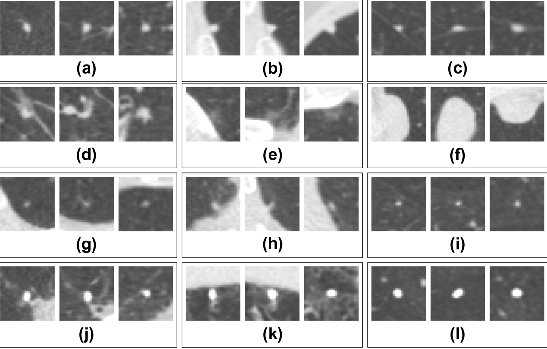
\includegraphics[width=\linewidth]{img/vanginnekennodules.png}
  \caption{In every box a nodule is shown in a sagittal, coronal and axial
  view. The diameter is provided between brackets. (a) isolated nodule (4,4
  mm); (b) pleural nodule (4,2 mm); (c) peri-fissural nodule (4,8 mm); (d) nodule with vascular
  attachments (5,9 mm); (e) ground-glass nodule (5,4 mm); (f) large pleural
  nodule (18,4 mm); (g) small nodule (3,2 mm); (h) small nodule (3,5 mm); (i)
  small nodule (2,3 mm); (j�l) shows three examples of bright, calcified nodules
  (indication of benign nodules)}
  \label{fig:nodules}
\end{center}
\end{figure}
The types of nodules stated above can be categorised. Juxta-vascular
pulmonary nodules have significant connections to their neighbouring vessels.
Pleural tail nodules have only thin connections to the neighbouring pleural
wall. Well-circumscribed nodules on the other hand do not have a connection to
the neighbouring vessels and structures. Juxta-pleural nodules show some degree
of attachment to their neighbouring pleural surface \cite{kostis}.
\begin{figure}[htp]
\begin{center}
  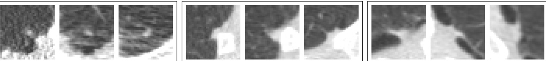
\includegraphics[width=\linewidth]{img/vanginnekenNonnodules.png}
  \caption{In the three boxes an apical scarring, a pleural thickening and a
nodular abnormality next to an emphysematous bulla are displayed in a sagittal,
coronal and axial view. These may be perceived by a nodule detection algorithm
as nodules, but in fact they are no nodules \cite{ginneken}.}
  \label{fig:Nonnodules}
\end{center}
\end{figure}
A number of nodule segmentation algorithms perform well in detecting specific
types of nodules. However, these CAD systems show large limitations in detecting 
for example non-isolated nodules that are connected to the pulmonary wall \cite{keshani}. 
These algorithms can be useful in particular situations, but if a detection 
algorithms really aims at being an asset for the radiologist, it should be able 
to detect all nodules while rejecting as much false positives (\autoref{fig:Nonnodules}) 
as possible.

\subsection{Overview of existing lung nodule detection systems}
As the demand for a reliable CAD system to detect pulmonary nodules is urgent, a
lot of research has been dedicated to the matter. Several commercial systems
have already been developed and many workstations that radiologists use to
examine CT scans offer on-board nodule detection or enhancement capabilities
\cite{ginneken}. However, although a lot of efforts were made, the results shown
in the various studies are rather diverse.

\subsubsection{Commercial systems}
In 2004 iCAD, Inc., provided lung cancer detection, analysis and tracking
software for the TeraRecon's Aquarius product line. The latter licensed several
software modules from iCAD. The iCAD QuickCue\texttrademark{} automatically
detects cancerous lung nodules. The iCAD QuickMatch\texttrademark{} locates,
compares and tracks nodules in previous or subsequent patient studies
\cite{tera}. However, the ImageChecker CT{}\texttrademark{}, launched by R2
Technology Inc., was the first CAD system approved by the US Food and Drug
Administration (FDA) for the detection of lung nodules during the examination of CT scans
\cite{Mevis}. In 2005 R2 Technology introduced the second-generation
ImageChecker CT Lung Version 2.0 CAD system which also implemented the AutoPoint
temporal comparison algorithm. This CAD system ``highlights abnormalities'' and
compares new and past images to demonstrate changes that have occured over time
\cite{diag, r2}. In 2006 Vital Images, Inc., and R2 Technology announced
the implementation of the R2 Technology's ImageChecker CT Lung CAD software into
the Vitrea workstations \cite{vital}. In the same year another company, Hologic,
Inc., acquired R2 Technology and implemented their CAD technology
\cite{Hologic}. Then, in 2008, MeVis Medical Solutions AG, Inc., acquired the
Pulmonary Computed Tomography Business from Hologic R2, Inc. \cite{Mevis}.

Although the technology from R2 Technology is in high demand, some companies
have developed their own software. In 2007 Medicsight plc, Inc., announced it
was granted a medical device license from the Therapeutic Products Directorate
of Health in Canada to introduce Medicsight LungCAD API\texttrademark \cite{HI}.
Another company, Median Technologies Inc., offers the LMS-Lung and LMS-Lung /
CAD modules which provide quantification and detection functionalities for
pulmonary (solid) nodules and micronodules \cite{median}. Siemens on the other
hand has developed the syngo.CT Lung CAD\texttrademark{}. They claim it is ``a
fully automated computer assisted second reader tool'' that is designed to
assist radiologists in the detection of solid pulmonary nodules \cite{siemens}.

\subsubsection{Publications of automated lung detection systems}
Apart from these numerous commercial systems many academic research
centers have tried to come up with a successful pulmonary nodule detection
system. \cite{review} suggest that most CAD systems for the automated detection
of lung nodules proceed according to a number of steps of which the first one is
the acquisition of data. The detection of lung nodules is preferably performed
on CT scans as they enable the visualisation of small volume and low-contrast
nodules because of the limited slice thichness. A large number of chest CT scans
are available in public databases such as the LIDC/IDRI database. In the next
step, the data are pre-processed to remove noise and artefacts which improves
the quality of the images, but it is not necessary to do so. In the third step a
segmentation of the lungs is performed. The lung lobe region is identified and
the rest of the image is removed. This reduces the computational cost compared
to the case where the whole image is processed and it increases the reliability
and the accuracy of the algorithm. The next step is the nodule detection. ``Lung
nodule detection refers to the process of determining whether nodule patterns
are present in the image and identifying the location of the nodules''
\cite[p.~154]{review}. Nodule detection methods can be categorized according to
the detection method that is applied. The first group of publications uses a
template matching technique to detect specific geometries. A second group relies
entirely on the output of a lung nodule segmentation method. The third group
applies a classification technique to classify voxels or regions of interest
(ROI). In addition, a clustering method may be implemented to improve the
performance of the system. The systems that include a classification component
in their nodule detection algorithm have demonstrated better performances
\cite{review}. In the final step of the process, the amount of false positives
is reduced to achieve a maximum sensitivity.

The first problem that arises when processing CT scan in search for nodules is
that one has to rely on the annotations made by expert radiologists. Accurate
delineation of these lung abnormalities is crucial for optimal image analysis.
The current approach to obtain delineations of lung nodules in CT scans involves
one or more radiologists manually drawing the boundaries of the nodules. Often
this manual segmentation overestimates the nodule volume to ensure the entire
lesion is enclosed \cite{rex}. Furthermore, this process shows a high inter- and
intrareader variability \cite{cooper}. But the success of the extraction of
image features depends on the accurate delineation of the nodules. Therefore, it
is of utmost importance this delineation is done in an accurate and reproducible
way. \cite{gu} have improved the ``Click and Grow'' algorithm that has been
developed by Definiens AG and Merck and Co., Inc., which semi-automatically
isolates tumors in CT images. The idea is that a radiologist detects the nodule
and clicks on the region of interest in a 2D slice. This click initiates
multiple seed points in a certain area. Then the application builds out the
object three-dimensionally by region growing. An ensemble segmentation is
obtained from the multiple regions that were grown. An evaluation on a set of
129 CT scans using a similarity index (SI) was performed.
The average SI was above 93\% which shows stability of the algorithm. The
average SI for two different readers was 79,5\%.

Apart from improving the manual nodule delineation of the radiologists, an image
processing algorithm may also increase their detection rate by assisting as a
``second reader''. \cite{roos} assessed the diagnostic performance of
radiologists -- with their years of experience ranging between 9 and 24 years --
and their temporal variation using incremental CAD assistance. 20 scans
containing 190 non-calcified nodules with a magnitude of 3 mm and above were
examined by three radiologists. After a free search, the radiologists
independently evaluated a number of CAD detections per scan. The average
sensitivity of their free search was about 53\% (range, 44\% - 59\%) at 1,15
false positives (FP) per scan. This increased up to 69\% (range, 59\% - 82\%)
and a FP rate of 1,45 per scan when using the CAD assistance. The increase in
sensitivity, with only a minimal increase in FP, was significant during a time
period of 100 seconds. Then the increase in sensitivity flattened from 14\% to
only 2\%. This evolution was due to the fact that the CAD nodules were presented
to the radiologists in order of CAD score and was not due to a temporal change
in the readers' performance. It was also noticed in this study that
different readers may experience a variable benefit from the use of CAD as some
readers tend to often reject true positive CAD candidates. This reduces the
potential benefit of CAD assistance. Nevertheless, \cite{roos} states that CAD
has the potential to equalise performance among readers by reducing individual
detection errors.

\cite{elbaz} proposed a three step algorithm to isolate lung nodules from spiral
chest low-dose CT scans. In the first step the lung tissues were isolated by
applying an iterative Markov-Gibbs random field (MGRF) based segmentation
framework. To retain the nodules attached to the pulmonary walls, the
segmentation was refined by the iterative conditional mode relaxation that
maximizes a MGRF energy. Then the lung nodules, arteries, veins, bronchi and
bronchioles were separated from the rest of the tissues in the slice. In the
second step the lung nodules (2-12 mm) were detected by applying 3D and 2D
templates which describe typical geometry and greylevel distributions within
nodules of the same type. Four template shapes were used: solid sphere, hollow
sphere, solid circle and solid semicircle. The radius and the greyscale
intensity of the templates were made adaptable. The detection combined the
normalized cross-correlation template matching and a genetic optimization
algorithm. The third step eliminated the FP using three textural and geometric
features that were calculated for each detected nodule.
To distuingish between FP and true positives (TP) Bayesian supervised classifier
statistical characteristics from a training set (20 FP, 20 lung TP, 20 lung wall
TP nodules) were selected from 50 separate subjects. CT scans from 200 subjects
were tested in this study and a sensitivity of 82,3\% and a FP rate of 9,2\%
were reached. The algorithm, that was implemented in C++ on an Intel Dual Core
processor with 16 GB memory, took about 5 minutes to process 182 CT slices of
size 512 x 512.

Other studies rely on a nodule segmentation method to detect lung abnormalities.
\cite{kuh} applies morphological opening, erosion, thresholding, seed
optimisation and boundary refinement operations to extract large nodules.
\cite{itai} proposes a segmentation of the lung areas using SNAKES method which
is an active contour model. Abnormal shadow areas over the size of 5 mm are
classified by using voxel densities. The algorithm was applied on 9 CT scans and
a TP fraction of 0,8 and a false negative (FN) fraction of 0,2 were obtained.

A third category of nodule detection methods are the classification based
methods. The main difference in output between a classification based detection
method and a segmentation method is that the latter will provide the user with a
delineation of the entire nodule, while the former will give a
nodule-probability per voxel. \cite{ozekes} tested four different learning based
classification methods: a Neural Network (NN) classifier, a Support Vector
Machine (SVM) classifier, a Naive Bayes classifier and a logistic regression
classifier. First a number of ROI were extracted by applying thresholding and an
8-directional search in which candidate lung nodule voxels had to have
neighbour voxels with densities between a minimum and maximum density threshold.
From these ROI a number of features were extracted: straightness, thickness,
vertical and horizontal widths, regularity and vertical and horizontal black
pixel ratios. These features were then fed to the four classifiers. The NN
classifier showed the best results, followed by the SVM classifier.
\cite{keshani} also applied a SVM classifier. The lung area was first segmented
by active contour modelling, which was followed by a set of masking techniques
to transfer nodules from non-isolated into isolated ones. Based on a set of 2D and 3D features the
SVM classifier was able to detect the lung nodules. Then the contours of these
nodules were extracted by active contour modelling. In a last step the lung tissues in
the original image were classified into four classes: lung wall, parenchyma,
bronchioles and nodules. The results from this classification were used to
distinguish solitary nodules from attached ones. When this algorithm was used to
detect nodules in the ANODE09 dataset an average detection rate of 37,8\% was
obtained while the best performing method yielded a detection rate of 63,2\%.
The latter algorithm, ISI-CAD, was developed by \cite{mur} and used the local
image features -- shape index and curvature -- to detect candidate nodules. Two
successive k-nearest-neighbour (K-NN) classifiers were applied to reduce the
number of FP. This yielded a sensitivity of 80\% with an average of 4,2 FP per
scan. \cite{sluimer2003} also used k-NN for developing an algorithm which
automatically distinguishes between normal and abnormal lung tissue.
Before the k-NN was applied, a principal texture analysis was performed in this
study to determine local features.

In addition to applying a classification based detection method, a clustering
method can be implemented as well to improve the performance of the classifier.
\cite{kawata} developed a linear discriminant classification boosted by k-means
clustering to distuingish between malignant and benign nodules based on
topological histogram features. The k-means clustering divided the datasets of
nodules in homogeneous classes to improve the performances of the linear
discriminant classifier. \cite{lee2010} also applied an ensemble classification
aided by clustering (CAC) method. First, nodule and non-nodule parts of a
training set were merged and then clustered into M clusters to take advantage of
the similarity among features of nodule and non-nodule instances. Then each
cluster was again divided into two groups, namely nodules and non-nodules. A set
of multi-class classifiers was then trained. The classifiers used were a Random
Forest (RF) classifier, a SVM classifier and a Decision Tree (DT) classifier.
There were two different clustering methods applied: k-means and expectation
maximisation (EM). The best results were obtained by the RF CAC EM algorithm. It
yielded a classification accuray of 97,72\%, while SVM and DT CAC EMs recorded
96,46\% and 93,98\% respectively. However, the execution time of the SVM CAC EM
algorithm was the lowest (182 seconds). These results were compared to non-CAC
methods. A classification accuracy of 95,64\%, a sensitivity of 95\%,
a specificity of 96,28\% and a FP rate of 3,72\% were obtained by non-CAC RF.
This method recorded the lowest execution time (10 seconds).


\subsubsection{Performance of existing systems} \label{sec:performance}
 The algorithms presented in a wide range of papers report varying degrees of
 success in the automated detection of nodules. However, it is very difficult to
 compare studies against one another in a meaningful way due to differences in
 the size of the datasets, the evaluation methods, the data selection criteria
 and the characteristics of the nodules under examination \cite{lee2010}.
 Especially comparing older and contemporary studies is difficult as older ones
 may have used scans with thicker sections (range 2.5 - 10 mm), on which small
 nodules are rather difficult to detect, than the scans nowadays (2,5 mm)
 \cite{lee2010, ginneken, mur}. Some studies focus on nodules below or above a
 certain size or on special types of nodules (e.g. solid nodules). \cite{mur}
 performed an extended literature review and found that the number of scans used
 for testing varied between 5 and 500 with a median number of 29,5. Many of the
 studies included multiple scans from individual patients, which means that the
 diversity of the available nodules was reduced. Furthermore, the results of
 publications are often presented in diverse ways.
 
 In order to improve the access to data, and thereby the comparability between
 studies, the Lung Image Data Consortium (LIDC) created a publically available
 database which provides researchers with a vast amount of test- and
 trainingsdata. Nevertheless, as one can take different subdatasets from this
 large database, it is still difficult to compare results in an objective and
 meaningful way. Therefore, \cite{ginneken} created ANODE09, a database of 55
 scans and a web-based framework which allows researchers to test their
 algorithms and to compare results against one another.
 





%voeg hier extra sections toe

\section{Methodology}
\subsection{Acquisition of the datasets}
The LIDC/IDRI database consists of 1018 thoracic CT scans that are obtained from
a heterogeneous range of scanner models (seven GE Medical Systems LightSpeed
scanner models, four Philips Brilleance scanner models, five Siemens Definition,
Emotion, and Sensation scanner models and one Toshiba Aquilion scanner model).
The database includes only one scan per patient so the scans are not correlated.
The nodules in the scans were delineated by at least four different expert
radiologists to identify as much nodules as possible. For this purpose the
indentification process was also subdivided into two phases: a blinded read
phase and an unblinded read phase. During the initial blinded read phase each
radiologist independently reviewed all scans and indicated the nodules in the
range of 3 to 30 mm and nodules smaller than 3 mm (if not clearly benign).
In the subsequent unblinded read phase the anonymized blinded read results of
all radiologists were revealed to each of the radiologists who then
independently reviewed their marks along with the anonymous marks of their
colleagues. The delineation of the nodules was done completely manually or in a
semiautomated way. This was allowed as a study on this topic showed that the
variation in nodule delineation done by different radiologists substantially
exceeded the variation derived from different software tools \cite{lidcbase}.

50 CT scans were obtained from the LIDC database \footnote{Freely available
at \url{http://cancerimagingarchive.net}.}. 12 scans were removed as they only
contained 1-voxel nodules. The pixel size of the scans varied between 0,586 and
0,963 mm and the slice thickness varied between 1,25 or 2,50 mm. This means the
diameter of the annotated 1-voxel nodules was less than 1 mm (micronodules).
These nodules are difficult to detect for a radiologist, especially if they are
hidden in a maze of vessels of the same magnitude. Therefore, some databases do
not require the radiologist to mark such small findings. In the Nelson Trail
database for example the radiologists do not have to mark nodules of which the
volume calculated by the Siemens LungCARE workstation software is less than 15
$mm^3$ \cite{mur}. This volume corresponds to a sphere with a diameter of about
3 mm, which is obviously more the 1 mm diameter from our 1-voxel nodules.
In the LIDC/IDRI database there were no limitations set on the diameters of the
nodules to be marked. However, the chance the radiologists marked every single
micronodule is very small. The training of the CAD algorithm can therefore not
be done properly as the annotations of the datasets are most propably incomplete
for nodules with a diameter less than 1 mm. Therefore, the datasets containing
only 1-voxel micronodules and the annotations of 1-voxel nodules in the
remaining datasets were removed. Furthermore, focussing on the detection of
these micronodules limits the level of thresholding that can be performed during
the classification of the datasets. Retaining these micronodules would prevent
us from eliminating a substantial part of the false positive findings. So
after eliminating these 38 scans remained for training and testing.
The RF algorithm was trained and validated on 30 and 8 CT scans respectively,
consisting of 5168 and 1249 slices with a average of 172 and 156 slices per
scan. Together with the original DICOM images the associated XML files
were obtained. These XML files provided a set of characteristics for each nodule
found: region, subtlety, spiculation, internal structure, lobulation, shape
(sphericity), solidity, margin, and likelihood of malignancy \cite{lidcbase}.
The trainingsdataset contained 64 nodules with each nodule containing 150 voxels
on average. The minimum and maximum radii of the annotated nodules was 2 mm and
18 mm respectively. The testdataset contained 19 nodules.


\subsection{Preprocessing of the data}
The initial exploration of the data and the generation of a mask to perform a
lung segmentation were done in MeVisLab 2.5.1 (VC11-64) (MeVis Medical Solutions
AG, Bremen, Germany). Further processing of the data and the implementation of
the RF algorithm were carried out in Python 2.7.6 (Python Software Foundation,
Delaware, U.S.A).  The training and testing of the RF based algorithm was
performed on a computer with Intel Core2 DUO CPU (2,27 GHz) and 3 GB of RAM.

\subsubsection{Processing of the annotations}
%convention: x,y,z = pixel, X,Y,Z = world

The annotations were partially provided in pixel coordinates -- x and y values
-- and partially in world coordinates -- Z values -- so the Z coordinates were
converted into pixel coordinates to find the nodule regions. The annotations
contained a list of x and y coordinates to indicate the position of each pixel
belonging to the contour of each nodule per slice. From these coordinates the
center of gravity plus the minimum and maximum radius of each nodule was
calculated per slice. The 1-voxel nodules were removed from the list of
annotations. In the rest of the algorithm each nodule was represented by its
center of gravity and its minimum radius.

\subsubsection{Lung segmentation}
It was assumed that, if the whole 3D scan was fed to the cascaded classifier,
only the soft tissue would remain after the first cascade. The grey value of
each voxel was used as a feature on this first level. Unfortunately, this method
did not prove to be efficient, so a second option was taken into consideration:
a proper lung segmentation as a preprocessing step.

By performing a lung segmentation, the amount of voxels that have to be
processed further on is significantly reduced by about 85\%. Furthermore, it has
the advantage that the soft tissues outside the lungs are eliminated so the
accuracy of the nodule detection system is increased. Therefore, it is the first
step that is performed in a lot of papers \cite{keshani, elbaz, teramoto}. We
started with implementing a lung segmentation algorithm based on \cite{keshani}.
The first part of this algorithm consists of obtaining a binary lung CT image by
adaptive fuzzy thresholding. In the binary image the lungs and the background
are separated from the soft tissues of the body.
Then two windows of different sizes are applied to close all the gaps in the
mask and the initial lung mask is obtained by sweeping a rotated window over the
entire binary image.
This sweeping is necessary to transfer non-isolated nodules into isolated ones.
Finally the mask is used to initiate an active contour model automatically for
segmenting the lung area. As stated the first step of this algorithm was
supposed to provide us with a variable, but accurate threshold to make the
binary image. The performance of this first step was assessed by applying the
algorithm on 42 slices -- 28 slices with lungs and 14 without lungs -- equally
distributed over 7 scans. The results varied among the scans. In some cases the
algorithm selected the appropriate threshold, in other cases the soft tissue
around the lungs was not eliminated well. Furthermore, performing the lung
segmentation as was described above would take a considerable amount of time
(minutes). Instead, a fixed threshold of 1600 was empirically established to
perform a body segmentation and to separate the soft body tissues from the rest
of the image. This is permitted because CT scanners have a carefully calibrated
output. Then gaps (lungs) in the body mask were closed by hole filling so a mask
of the entire body was obtained. As this body segmentation already eliminated
55\% of all voxels and no complex calculations had to be done to obtain the
binary image, this result was found satisfying enough.

Despite the reduced amount of voxels, applying the algorithm still raised memory
errors depending on the dimensions of the scan.
In order to reduce the amount of voxels even further in the pre-processing
phase, a full lung segmentation was performed in a semiautomatic way in
MeVisLab. After the scans were loaded in MeVisLab, the user manually indicates
three points inside the lung area. Based on these points region growing is
performed and a binary mask for the lung area is generated. The gaps in the
binary mask -- which represent nodules in the lung area and nodules hidden in
the lung wall -- are closed by dilation. This mask is then exported to Python
for further processing of the images. 

An alternative way of performing a lung segmentation in Python would be
calculating the body mask at the fixed threshold of 1600 and subtracting this
mask from a similar mask in which the lung gaps are closed. In this way only the
lung area is retained. Then a dilation and erosion should be performed as well
to include the nodules hidden in the lung wall.

\subsection{Training of the classifier}
\subsubsection{Preparation of the training dataset}
Based on the associated annotations the center of gravity, the minimum and
maximum radius of each nodule was calculated. With this information a sphere
was constructed which comprised the whole nodule. To select the central volume
of the nodule, one third of the radius was taken as an artificial boundary. Only
the voxels in this center were considered further in the process as voxels
belonging to a nodule. Reducing the amount of positive voxels -- voxels
comprised by a nodule -- was done to avoid taking into account the ambiguous
edges of the nodules. These edges might confuse the classifier. As the aim of
this project was not to delineate entire nodules but assigning nodule
probabilities to the voxels in the image, this reduction in order to provide
clear training data for the classifier was justified.

However, instead of a sphere -- which defines the nodules in 3D -- this concept
was applied per slice as it was noticed that the delineation of the nodules was
not always done properly so a lot of nodules showed a flattened shape
(\autoref{fig:flatNodule}).
Therefore, the minimum radii of the nodule in each slice were separately
determined and two third of these radii was taken to select the central volume
of the nodule. A list of positive voxels per scan was constructed this way.
\begin{figure}[ht]
 \begin{center}
    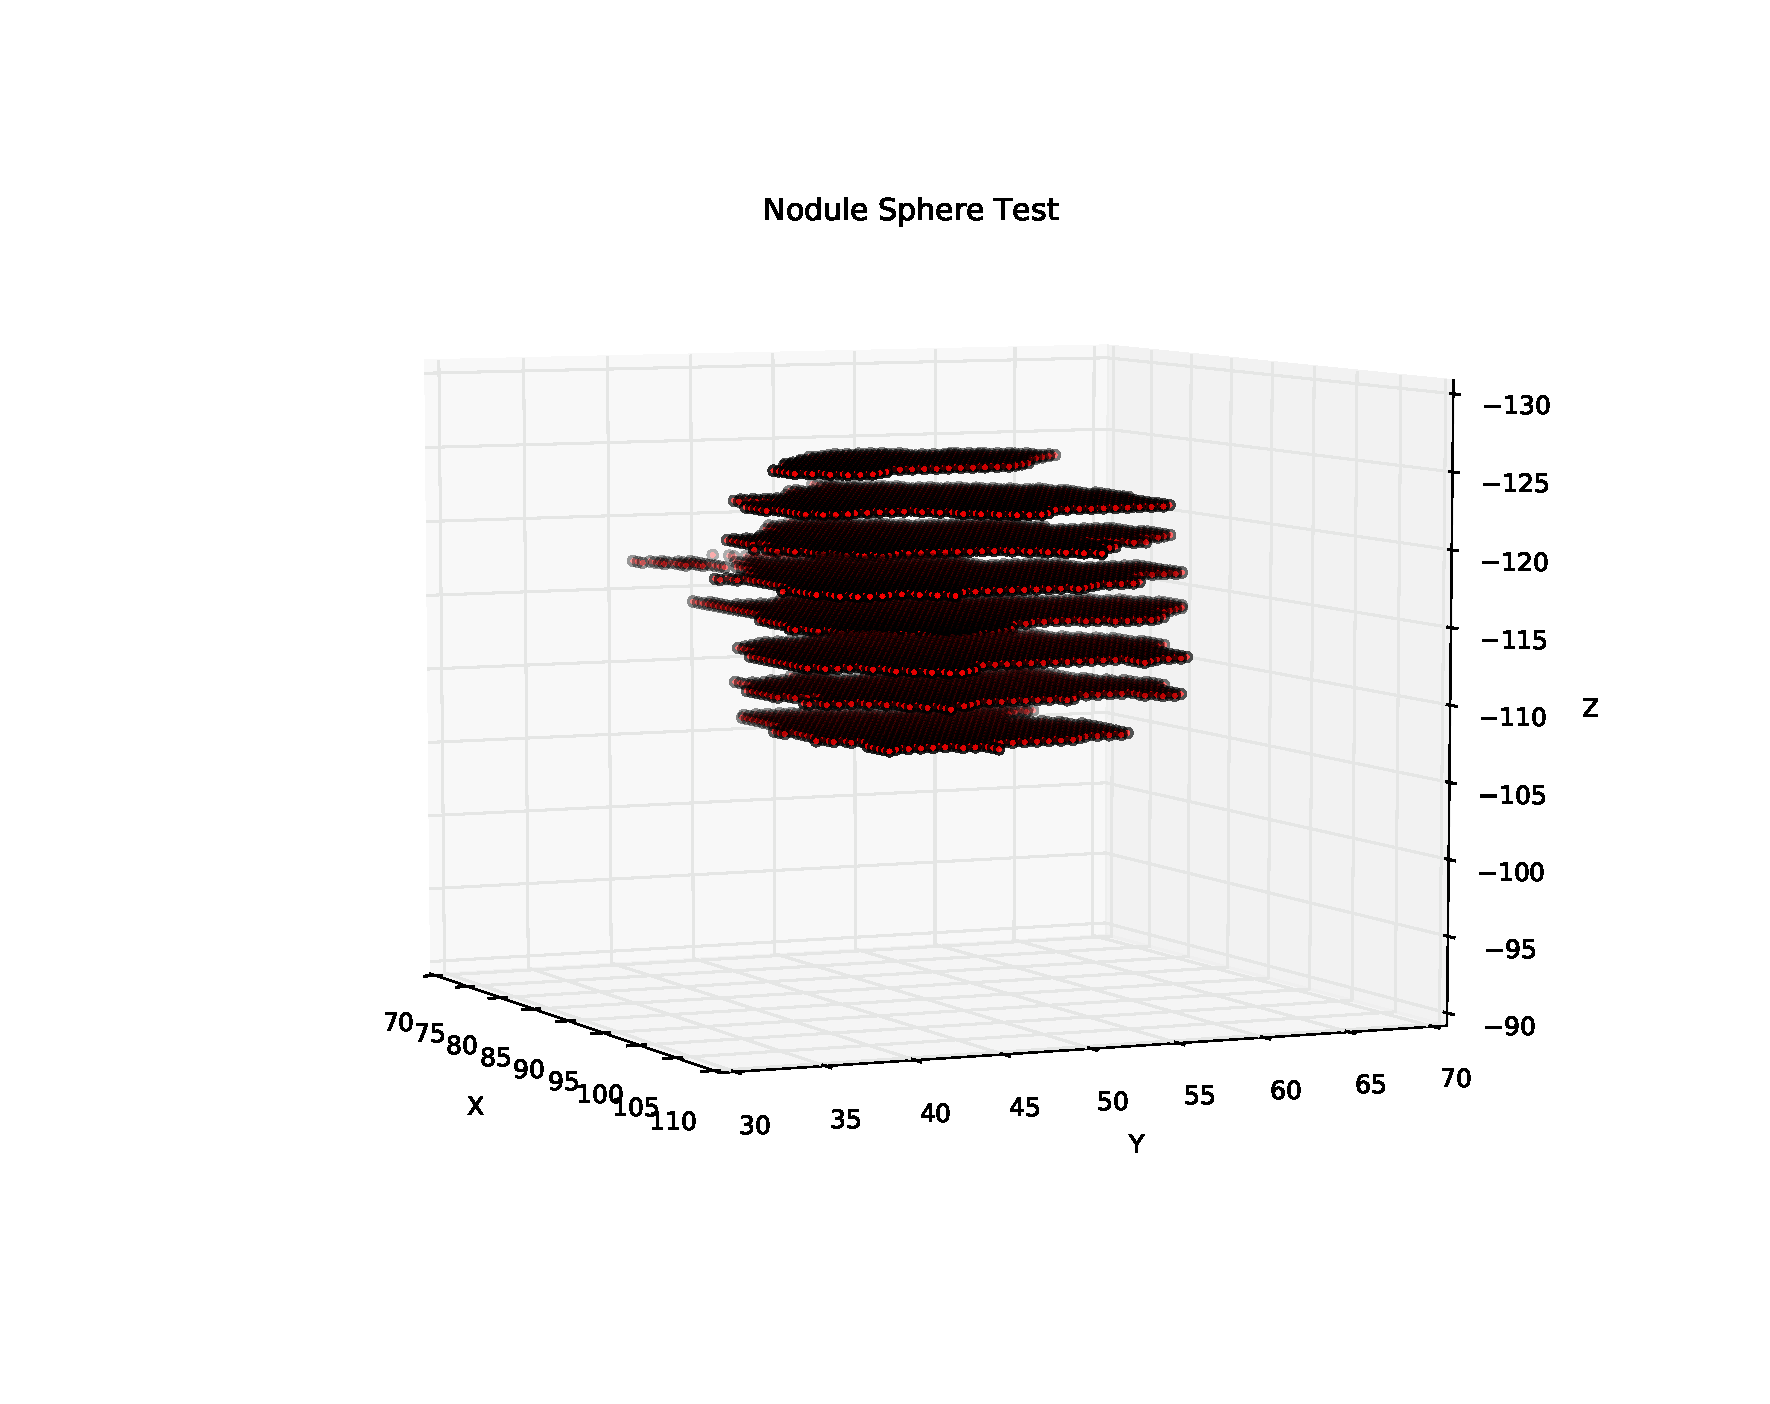
\includegraphics[width=\linewidth, trim=150 0 0 0]{img/NoduleSphereTest_0001.pdf}
    \caption{Flattened shape of nodule (LIDC scan 0001)}
    \label{fig:flatNodule}
 \end{center}
\end{figure}

To train a classifier, a list of positive and negative
examples are necessary. Therefore, a second list of voxels was constructed. The
amount of voxels was taken the same as in the list of positive voxels to obtain
a balanced training dataset. The positions of the negative voxels were selected
at random over the entire image. The only constraint was that they were not
allowed the be situated within two times the maximum radius of each nodule. This
constraint was imposed to avoid ambigous training data.

Then features were calculated for both the positive and the negative voxels. The
features that were used are discussed in section \ref{sec:featureExtraction}.
This resulted in a list of features and a class (nodule or non-nodule) per
voxel. This whole process was repeated for all scans and the results were then
concatenated to obtain a dataset to train the ensemble classifier. We summarized
it using pseudocode in algorithm \ref{alg:train}.

\begin{algorithm}[ht]
	\DontPrintSemicolon
	\caption{Training Phase\label{alg:train}}
	\ForEach{$dataset \in trainingsets$}{
		load DICOM files\;
		load XML annotations\;
		\ForEach{$nodule \in annotations$}{
			\ForEach{$slice \in nodule$}{
				select positive voxels ($d < 0.66R_{min}$)
			}
		}
		\While {negative pixels $<$ positive pixels}
		{	select random pixel in volume\;
			\If{not near nodules ($d > 2R_{max}$)}{
				select negative voxel
			}
		}
	}
	\For{level from 1 to max}{
		\ForEach{selected pixel}{
			generate feature vectors up to level\;
		}
		train classifier\;
		save classifier model\;
	}
\end{algorithm}

\subsubsection{Feature extraction and selection} \label{sec:featureExtraction}
\paragraph{Features implemented in final algorithm}
The \textbf{grey value} of each voxel is the only feature of the cascaded
classifier at level one. From this, the classifier learns that nodules are
always part of the soft tissue window. When asked to identify nodules with this
information alone, the classifier will simply highlight all soft tissue in the
image. Remember that during the preprocessing we applied a lung mask. Hence all
soft tissue outside of the lungs -- save for a thin edge caused by dilation --
is already discarded. By combining the two results, we are left only with thin
lung edges, nodules and bronchi/bronchioli. The task of the next classifiers in
the cascade will be to further distinguish between these different structures.

In level two, our focus goes to discarding the remaining lung edges and
highlighting the nodules. We do this by combining a LoG \textbf{blob detector}
with a \textbf{distance map}. As explained in section \ref{sec:laplace_theory},
the LoG operator is very good in detecting light blobs on a darker background
such as nodules. The remaining lung edges in contrast do not fit this
description at all. To find out which sigma would work best, we performed a
couple of tests. First, we know that larger sigmas work better on larger nodules
and vice versa. To that end, we searched for the smallest and largest nodule
over all our datasets. Next, we empirically established the sigmas that yielded
the best results for each. Because we do not know ahead of time how big the
nodule we have to detect will be, we calculate the LoG for all intermediary
values. The results of our test (see figure \ref{fig:radii}) show that nodules
radii lie between 2.68 mm and 18.39 mm with a mean of 6.32 mm and that
we need sigmas between 2mm and 10mm to cover this range.

\begin{figure}[ht]
\begin{center}
  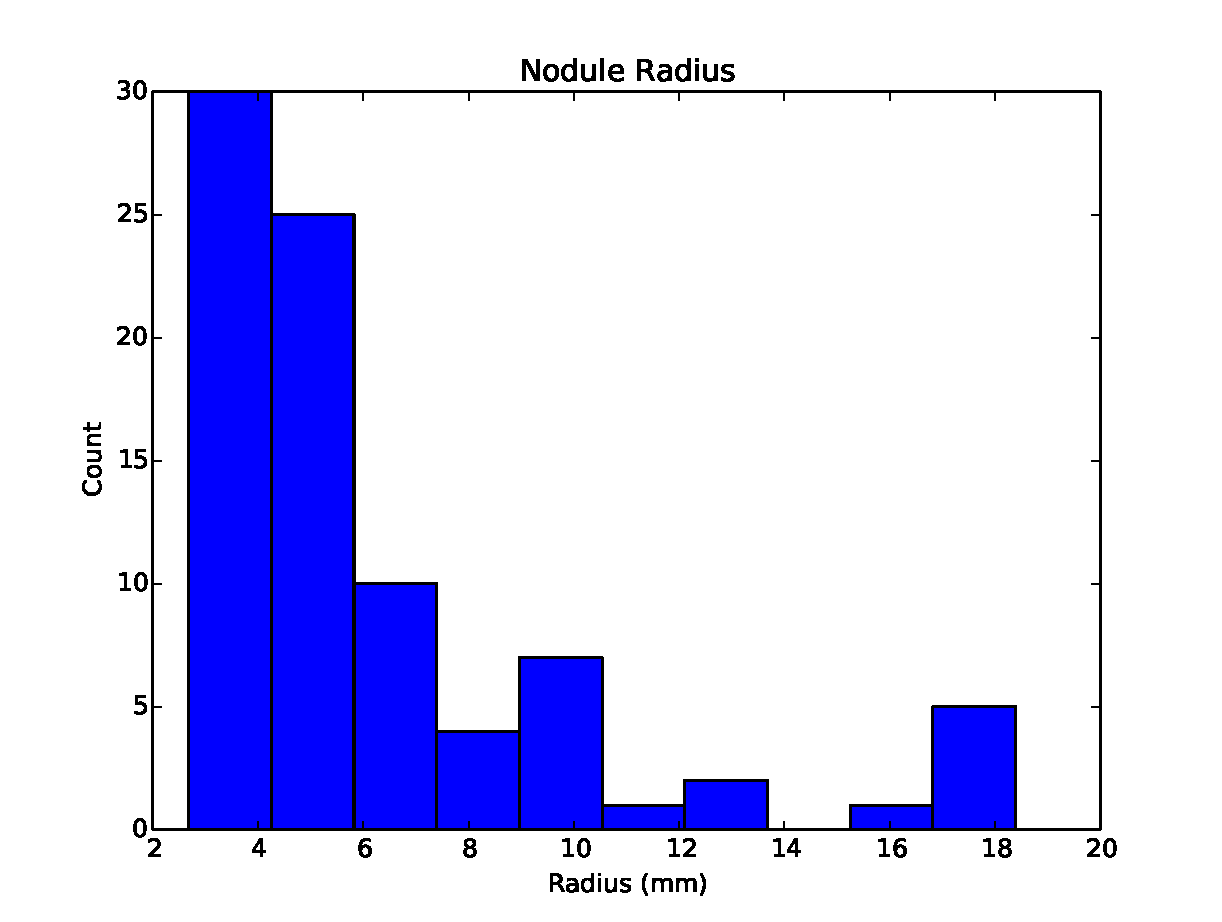
\includegraphics[width=\linewidth]{img/MaxNoduleRadii.pdf}
  \caption{Histogram of nodule radii}
  \label{fig:radii}
\end{center}
\end{figure}

To make the difference even more clear to the classifier, a distance map was
calculated based on the original lung mask. Alternatively, one could also work
with an ordinary edge detector, e.g. sobel. By blurring that output with a
Gaussian, we get a similar distance-to-edge feature. However, we chose the
distance map over this approach because it simply contained more information. Of
course we can't blindly discard any voxels too close to the edges, because
nodules can be closeby as well. That is why a distance map alone is not enough.

At the third and fourth level \textbf{3D averaging} was implemented to get rid
of the bronchi and bronchioles that were still present. See section
\ref{sec:3davg} for more information. With the help of all the features above,
the classifier should have enough information to separate the nodules from other
structures in and around the lung.

\paragraph{Experimental features}
This paragraph provides an overview of other features that were
tested but that were not implemented in the final classifier.

The \textbf{skewness and kurtosis} of a 3D window around each
voxel was calculated as a measure for the texture of a certain part of the image. The
skewness is a measure of the asymmetry of the probability distribution
distribution of a real-valued random variable (grey value) about its mean. The
kurtosis is a measure of the peakedness of the probability distribution of a
real-valued random variable. However, the implementation of these first order
statistics in the final classifier was prohibited by the time needed (hours) to
calculate these features for every voxel in the image.

Another obvious feature, apart from the grey value of each voxel, is the
\textbf{position} $(X, Y, Z)$ of each voxel in the 3D image. An even better
feature is the \textbf{relative position} $(\tfrac{X}{X_{max}},
\tfrac{Y}{Y_{max}}, \tfrac{Z}{Z_{max}})$ as it takes into account that the size
of the datasets might change. These features could be useful when lung
segmentation is not performed, because they could limit the search area.
However, after testing it showed that these features would only be useful if a
very large amount of training data was used. Figure \ref{fig:posFeature} shows
what happens when only 10 datasets are used to train such a classifier. The
training set had to be large enough so almost every possible nodule position
inside the lungs was covered by the training data. This would not only be very
inefficient, but interpersonal differences in lungmorphology would make it even
more difficult. Hence the features 'position' and 'relative position' were
exluded from the feature set.
Instead a distance map based on the lung mask was implemented as a feature.

\begin{figure}[ht]
\begin{center}
  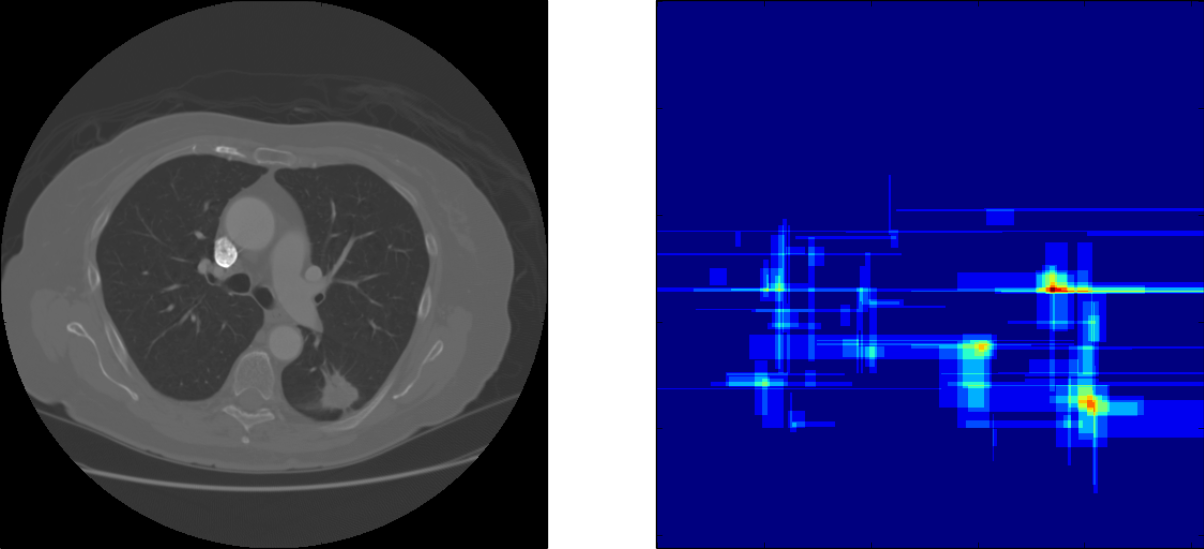
\includegraphics[width=\linewidth]{img/RelPositionFeature.png}
  \caption[]{Probability output of a classifier trained on 10 datasets with only
  1 feature: relative position. The output simply highlights the positions of
  nodules encountered in earlier datasets, without being relevant for the
  currect dataset.}
  \label{fig:posFeature}
\end{center}
\end{figure}

A \textbf{3D Sobel filter} for edge detection was implemented as well. A Sobel
filter is typically a $3 \times 3$ convolution mask that approximates the
partial derivative of an image along an axis. The results of multiple sobel
filters can be combined to calculate the gradient magnitude of each pixel. A
high magnitude usually corresponds with an edge in the original image.

To be really useful in nodule detection, the distance from each voxel to
neighbouring edges had to be calculated. However, due to a lack of time this was
not feasible anymore. Instead, the distance map mentioned above was used as a
substitute.

The \textbf{entropy} of an image is a measure for the chaos of the image in a
certain neighbourhood. Low entropy images are images where vast areas of pixels
have the same grey values. Images with high entropy show a large contrast
between neighbouring pixels. Therefore, it is a measure for the texture of an
image. The entropy of the entire 3D image was calculated and then the values for
each voxel were extracted. However, the time demand for these calculations were
far from negligible and as a consequence this feature was eliminated again.

A feature \textbf{neighbours} calculated the sum, the subtraction, the
multiplication and the quotient of the voxel in front and behind, left and right
and above and below a target voxel. Each of these operations where also
performed with the target voxel itself and the neighbouring voxel. Another
substantial amount of features were based on calculations within \textbf{3D
windows} that were swept over the lung mask of the image. The same operations
as in neighbours were executed on a larger scale: the neigbouring voxels were
determined by a certain adaptable window around the target voxel. Except for
these basic operations the mean, the standard variance, the minimum and the
maximum of the grey values of each window were calculated. Then these parameters
and the grey value of the target voxel were used for performing the basic
operations (sum, subtraction, multiplication, quotient) on. The same idea was
applied on the rows and columns in each window. The mean of different rows and
columns were determined and compared to each other by means of summing them up,
subtracting them, dividing one by another and multiplying them. In these windows
a frequency count was performed for each grey value in the window. These
frequencies were again compared. The results that were obtained this way could
be compared to one another by comparing the results for subwindows within larger
windows or within the entire image. However, none of these features were
implemented in the final classifier as calculating features for each individual
voxel in an image took too much time (hours).

%\subsubsection{Training of the classifier}
\subsubsection{Cross validation}
During the training phase, we already want to get an idea about the future
performance of our classifier. Of course we could use the whole feature set in
the training, and use the same features afterwards to check if our classifier is
performing well. However, this is considered a form of cheating, and the test
would not tell us much about the predictive power of the classifier on new data.
That is why it is important to reserve a fraction of the feature vectors for
cross validation. A strategy called stratified K-fold is used to repeatedly
split the feature set randomly in a train and a test fraction.
The stratified adjective means that the proportion of nodules to non-nodules are
similar in both fractions. Each time -- also called \textit{fold} -- the
classifier is trained with the train fraction and performance is checked with
the test fraction. After a number of folds, these results are combined to give a
proper estimate of the classifier performance in terms of accuracy (or other
score metric).

This cross validation can also be used to determine the optimal hyperparameters
of the classifier. By generating a grid of parameters and corresponding value
ranges, all combinations can be tested, and the one with the highest score can
be retained. In case of RF, it is important to configure it in such a way that
overfitting does not occur. This can be done by increasing either the tree
depth, the minimum number of samples per leaf or the minimum number of samples
before a split occurs. The minimum number of samples per leaf was chosen to
perform the optimalisation with.

\subsection{Testing and validation of the classifier}
From the previous section, we obtained a trained RF model that can be used to
predict the class of new image features with a certain probability. We use this
facility for two purposes: feature effectiveness testing and output validation.
But before any of that can be done, features must be calculated for all
remaining voxels in the new dataset. A cascading approach allows us to do this
while keeping computational en memory cost acceptable. Additionally, a lung mask
is applied to the whole volume, allowing us to ignore any outside voxels from
the start.

To assess feature effectiveness, we ask ourselves the following question. Is a
substantial amount of non-nodule voxels removed from the dataset without
removing the nodule voxels as well, i.e. did the specificity increase without
affecting the sensitivity? If this is the case the feature is kept at that
level, otherwise another feature is implemented. The assessment is performed
based on a probability image that is generated by combining the resulting
probability output from all feature vectors. The first section of algorithm
\ref{alg:test} summarizes this procedure.

\begin{algorithm}[ht]
	\DontPrintSemicolon
	\caption{Testing \& Validation Phase\label{alg:test}}
	\ForEach{$dataset \in testsets$}{
		load DICOM files\;
		mask $\longleftarrow$ load lung mask\;
		\For{level from 1 to max}{
			load classifier model\;
			\ForEach{$pixel \in mask$}{
				generate feature vector\;
				probability $\longleftarrow$ classify\;
			}
			combine into probability image\;
			mask $\longleftarrow$ (prob. image $>$ threshold)\;
		}
		result = mask\;
		discard non-nodule voxels ($p < 50$\%)\;
		cluster remaining voxels\;
		load XML annotations\;
		\ForEach{$nodule \in annotations$}{
			\eIf{any cluster $\in$ nodule ($d < 1.5R_{max}$)}{
				$TP{+}{+}$\tcp*[r]{nodule detected}
				delete clusters\;
			}{
				$FN{+}{+}$\tcp*[r]{nodule not detected}
			}
		}
		\ForEach{remaining cluster}{
			$FP{+}{+}$\tcp*[r]{spurious cluster}
		}
		calculate statistics
	}
\end{algorithm}

When all features were decided upon, we validated the entire algorithm.
% 1 voxel clusters weg

\section{Results and discussion}
\subsection{Optimisation of the classifier parameters}
By performing a five fold cross validation during the training stage the most
optimal parameter set for the RF algorithm were discovered. It was found that
for all levels except the first, a value of 5 yields optimal results for the
minimum samples per leaf parameter. For level 1, this optimal value was
significantly higher at 55. This makes sense as higher values correspond to less
complex classifiers.

The accuracy that was reached was respectively 80,5\%, 97,9\%, 98,1\% and 98,2\%
for the four consecutive levels. This shows that the first two levels in the
cascade contributed more in the process of removing negative voxels than the
last two levels. The latter however were not useless as they still increased the
level of accuracy. The fourth level for example still eliminated about 600
voxels per scan. Though, as mentioned before, the accuracy metric should be
taken with a grain of salt in highly unbalanced classification tasks.

For each level of the classifier, a threshold was set to determine which voxels
would be passed on to the next level (i.e. which voxels showed a higher nodule
probability). In order to avoid discarding nodule voxels of small nodules a
rather low threshold had to be set. These were empirically determined at 20\%,
40\%, 40\% and 70\% for the four levels respectively, although more rigorous
testing might yield even better values.

\subsection{Validation results}
In this section, we will illustrate our results based on two slices from the
fiftieth LIDC dataset. The volume dimensions are $512 \times 512\times 139$ and
it contains one nodule around slice 95. As figure \ref{fig:d50} shows, slice 50
contains no nodules while slice 95 indeed contains exactly one. After applying
the lung mask, 13,59\% of all voxels remain.

\begin{figure}[ht]
\begin{center}
	\begin{subfigure}[b]{\linewidth}
		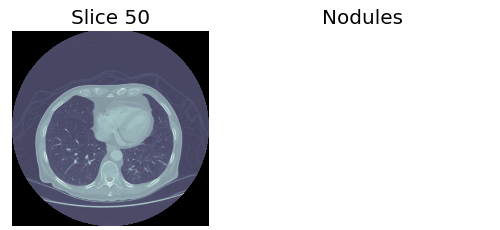
\includegraphics[width=\linewidth]{img/cascades/D50S50.png}
		\caption{Slice 50}
	\end{subfigure}
	\begin{subfigure}[b]{\linewidth}
		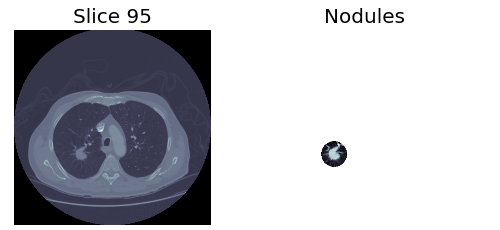
\includegraphics[width=\linewidth]{img/cascades/D50S95.png}
  		\caption{Slice 95}
	\end{subfigure}
	\caption{Example of two slices in dataset 50, one without and one with a
	nodule.}
	\label{fig:d50}
\end{center}
\end{figure}

\paragraph{Level 1}
As expected, we get a significant reduction in the number of voxels. More
specifically only soft tissue structures -- i.e. lung wall, bronchi/bronchioli
and nodules -- remain. The threshold performs a straightforward segmentation and
cannot be improved much.

\begin{figure}[p]
\begin{center}
	\begin{subfigure}[b]{\linewidth}
		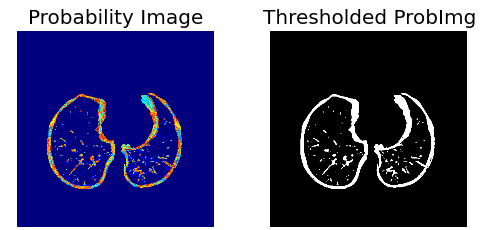
\includegraphics[width=\linewidth]{img/cascades/D50S50L1.png}
		\caption{Level 1 -- Threshold: 20\% -- 5,74\% remaining}
	\end{subfigure}
	\begin{subfigure}[b]{\linewidth}
		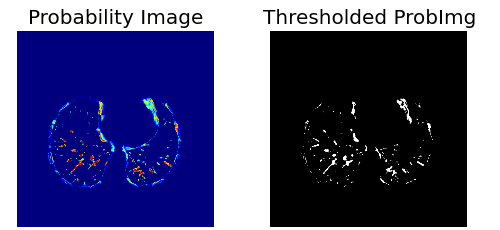
\includegraphics[width=\linewidth]{img/cascades/D50S50L2.png}
		\caption{Level 2 -- Threshold: 40\% -- 1,86\% remaining}
	\end{subfigure}
	\begin{subfigure}[b]{\linewidth}
		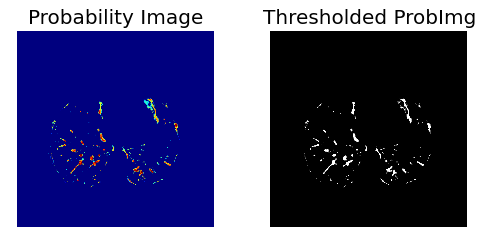
\includegraphics[width=\linewidth]{img/cascades/D50S50L3.png}
		\caption{Level 3 -- Threshold: 40\% -- 1,55\% remaining}
	\end{subfigure}
	\begin{subfigure}[b]{\linewidth}
		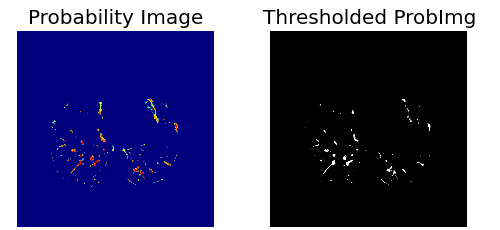
\includegraphics[width=\linewidth]{img/cascades/D50S50L4.png}
		\caption{Level 4 -- Threshold: 70\% -- 0,54\% remaining}
	\end{subfigure}
  \caption{Processed versions of slice 50 in dataset 50. Left: probability
  image. Right: threshold of probability image showing the voxels that continue
  to the next level in the cascade. The algorithm started with 13,59\% of all 
  voxels remaining after lung segmentation.}
  \label{fig:d50s50}
\end{center}
\end{figure}

\begin{figure}[p]
\begin{center}
	\begin{subfigure}[b]{\linewidth}
		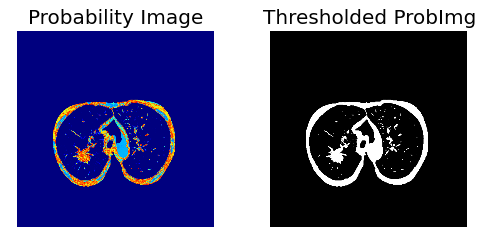
\includegraphics[width=\linewidth]{img/cascades/D50S95L1.png}
		\caption{Level 1}
	\end{subfigure}
	\begin{subfigure}[b]{\linewidth}
		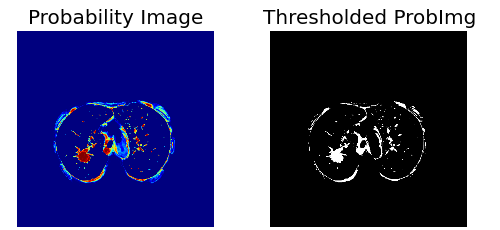
\includegraphics[width=\linewidth]{img/cascades/D50S95L2.png}
		\caption{Level 2}
	\end{subfigure}
	\begin{subfigure}[b]{\linewidth}
		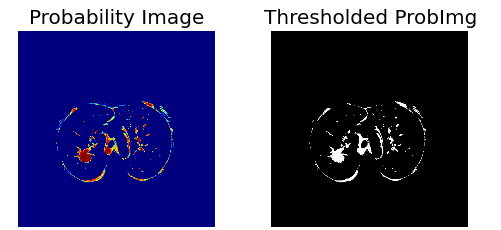
\includegraphics[width=\linewidth]{img/cascades/D50S95L3.png}
		\caption{Level 3}
	\end{subfigure}
	\begin{subfigure}[b]{\linewidth}
		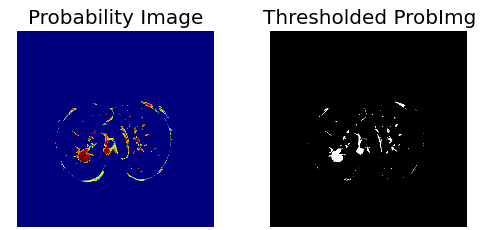
\includegraphics[width=\linewidth]{img/cascades/D50S95L4.png}
		\caption{Level 4}
	\end{subfigure}
  \caption{Processed versions of slice 95 in dataset 50. Left: probability
  image. Right: threshold of probability image showing the voxels that continue
  to the next level in the cascade. The same thresholds and remaining counts
  apply as in figure \ref{fig:d50s50}.}
  \label{fig:d50s95}
\end{center}
\end{figure}

\paragraph{Level 2}
This level was meant to highlight nodule-sized blobs while reducing the response
of other structures, in particular lung walls. The laplacian filter certainly
succeeded in the former, although we still get a medium-high response from
certain wall segments at times. Unfortunately, the laplacian also highlights the
smaller structures in the lung. This was inevitable as we needed LoG filters
with small sigmas to find small nodules. There is definitely room for
improvement in threshold level. A higher threshold could discard more wall
voxels while retaining nodules. In conclusion it is still a well performing
feature that significantly reduces the voxel count, although it has some
unfortunate side effects.

\paragraph{Level 3 and 4}
The goal here was to discriminate between small bronchioli and blood vessels on
the one hand, and small nodules on the other hand by means of 3D averaging.
Unfortunately, this feature does not perform as well as hoped: there is only a
margin decrease in non-nodule voxels. Note that the fourth level feature with
the larger internal threshold works slightly better, but still not satisfactory.
Future work should either fine-tune the parameters of this method or find a more
effective method altogether.

The obtained sensitivity of the algorithm was 100,00\% with an average of 2,17
TP and 4279,43 FP per scan. This high number of FP results in a very low
precision of 0,0634\%. Training the algorithm on 30 scans took 1 hour and 50
minutes. The processing of a new medium-large dataset (136 slices) takes about
10 minutes.

Keeping in mind that comparing different studies is difficult (see section
\ref{sec:performance}), some relevant results from literature are presented
here. \cite{teramoto} used a cylindrical nodule-enhancement filter and performed
a FP reduction using a SVM classifier. This method reached a sensitivity of 80\%
and 4,2 FP per LIDC/IDRI scan. The detection speed ranged from 25 to 34 seconds
per scan. \cite{elbaz} applied template matching and found a sensitivity of
82,3\% and a specificity of 9,2\%. The time to process 1 scan in C++ was about 5
minutes. \cite{lee2010} tested an ensemble classification aided by clustering
(CAC) method on a set of nodules and non-nodule examples and they obtained a
classification accuracy of 97,72\%. An execution time of 190 seconds was
registered.

These results indicate our algorithm performed well concerning detecting all
nodules, but the amount of FP has to be reduced to get the precision up. At the
moment, the algorithm is simply not strict enough: it detects all nodules but at
a high FP cost. This amount can be reduced in a first stage by determining
the optimal value for all parameters, such as the threshold for each cascade
level.

Our ``potential nodule'' clustering strategy also plays a significant role here.
By clustering individual voxels together we hope to make them more comparable
to nodules, but this is not always the case. Some clusters are simply too small
to even represent a realistic nodule. Filtering out these clusters will help
boost our results.

Another way of improving the algorithm is increasing the amount of training
data. To determine the optimal amount of datasets a trade-off should be made
between the time it takes to train the algorithm with extra datasets and the
diminishing marginal improvements in the performances of that action. 

A third possibility is implementing more features (e.g. Haar-like features),
especially features focusing on removing edges and eliminating the bronchioles.
On the other hand, implementing more features will increase the processing time.
However, by optimising the thresholds in the existing algorithm these things can
also be (partially) achieved. The threshold on level two can be set higher which
will remove more edges. For eliminating the bronchioles the parameters of the 3D
averaging features should be optimised. The results from the literature also
show that we have a long processing time. However, one has to take into account
that the implementation of this algorithm was done in Python -- an interpreted
language -- which makes it inherently slower than low-level compiled languages
such as C++. Nevertheless, Python was chosen for its rapid prototyping
abilities. Future work may implement our algorithm in C++ or another compiled
language to speed up the computational process.

\cite{ginneken} compared the performances of six nodule detection CAD algorithms
on the same validation dataset. The sensitivities at seven levels of false
positive detection were calculated and then averaged. The best performing method
in this study yielded an average sensitivity of 63,2\% for the detection of all
kinds of nodules. The sensitivity per nodule type was also provided: small
nodules (63,4\%), large nodules (62,8\%), isolated nodules (60,9\%), vascular
nodules (69,3\%), pleural nodules (43,5\%) and peri-fissural nodules (76,6\%).
This clearly shows that the ease of nodule detection also depends on the type of
nodule. As this information is not available in the annotations of the LIDC
scans and as we did not cooperate with a radiologist, it is not possible to
differentiate between the different types of nodules in this project. However,
as we may assume that different nodule types are represented in our testset, it
is clear the algorithm is able to detect several types of nodules except for
extremely small ones as we removed these from the annotations in the training
and validation phase.

%TODO suggest using cross validation for the 30-8 groups as well

\section{Conclusion}
CT technology has come to the point where high resolution images of the whole
chest can be obtained in a single breath hold. The resolution allows to detect
pulmonary nodules in an early stage and therefore CT scans become more and more
part of routine investigations. This causes a large increase in the workload of
the radiologists, who are only human and thus also prone to errors. Time
pressure and fatigue may lead to an increasing fraction of overlooked nodules.
Research showed however that pulmonary lung detection systems, that serve as a
second reader, can improve the performances of radiologists.
Therefore, the goal of this project was to develop an accurate, fast and
automated system to detect pulmonary nodules in CT scans.

A non-exhaustive literature review revealed that companies such as R2
Technology, Siemens, iCAD etc. already have invested in the development of
similar software. However, a satisfying allround software package does not exist
yet. The research is still ongoing to develop a system with 100\% sensitivity
and no false positives detection. One of the problems that arises here is that
there is no golden standard to measure the performance of the CAD system
against. Currently, the performances of CAD systems are compared with the
findings of one or more radiologists. Although the fraction of overlooked
nodules decreases when more radiologists cooperate when analysing a CT scan,
there is no guarantee that all nodules are delineated in a scan. This makes it
very hard to assess the performance of a automated nodule detection system.

There are three main schools of thought in the development of pulmonary nodule CAD
systems. The first group uses template matching to detect (a type of) nodules. A
second group performs a nodule segmentation by means of a series of
morphological operations, active contour modelling, etc. The third group applies
classification methods, possibly aided by clustering. As there is evidence
in literature that this method yields the best results, a more extensive
literature review was performed to select a proper classification method. It was
decided to use a cascaded Random Forest classifier as this type of classifiers
is not yet fully explored in this area of research. This provided the
opportunity to beat the state of the art in nodule detection algorithms.

Random Forests have many advantages. As an ensemble classifier it combines
decisions of multiple classifiers to form an integrated output. This way of
working has the advantage that a better predictive performance is obtained
compared to the predictive performance demonstrated by each individual learning
algorithm separately. Furthermore, Random Forests are rather robust against
noise compared with other classifier such as Support Vector Machines. Random
Forests also allow to use a lot of features, even if they have different orders
of magnitude, without increasing the time complexity too much. The features also
do not have to be known in advance. At the same time, the method does not
require a lot of parameter tuning. The only thing that has to be taken into
consideration is the depth of the trees as overfitting must be avoided in order
to maintain an algorithm that is able to generalise across datasets. The use of
a cascaded classifier is preferred as it limits the amount of CPU time and
memory storage.
 
The higher the level in the cascaded classifier, the more complex the features.
On the first level the grey values of the voxels were used to detect soft
tissue, to which class nodules belong. Although this first level is able to
eliminate the voxels outside the lungs, a lung segmentation was applied first to
reduce the amount of voxels to be processed. The reason for this were recurrent
memory errors when attempted otherwise. On the second level a blobdetector --
Laplacian filter -- and a distance map were implemented. On the third and fourth
level a 3D averaging algorithm was elaborated with two different
parametersettings. This 3D averaging allows to separate nodules from bronchioles
and bronchi by taking into account the presence of these structures in the
preceeding and/or succeeding slices. A lot of other features were implemented
and tested, but most of them were removed again from the final classifier as
they required a lot of processing time and did not perform accordingly. After
each level in the classifier a threshold was set to determine which voxels were
taken to the next level and which were to be discarded. These thresholds were
empirically determined, but can still be optimised. The training and the
validation of the algorithm were performed on 30 and 8 datasets respectively.

During the training of the algorithm a five-fold crossvalidation was performed
to determine the optimal set of parameters for the Random Forest algorithm. It
was decided to take into account the optimal number of minimum samples per leaf
to keep the algorithm from overfitting. An accuracy level of 98,2\% was achieved
in the last level of the cascaded classifier.

The validation of the optimised classifier showed 100\% sensitivity, but also
indicated the amount of false positives still has to be significantly reduced.
The processing time of 10 minutes per scan is not extremely satisfying, but one
has to take into account that Python is an interpreted language which makes it
inherently slower than for instance C++. Transferring the code to a compiled
language will speed up the process. The aim is to be able to process one scan
within a few minutes. There is no need for faster processing as a radiologist
will not need the results earlier, but it should not take much longer either.

The amount of false positives per scan (4279,43 FP per scan) has to be reduced.
A first step to achieve this is the optimisation of the thresholds in the
algorithm. A more accurate setting of the thresholds will also be possible if the
algorithm is trained on a larger amount of scans. On top of that, the clustering
strategy might have to be revisited. Another possibility is the implementation
of more features. However, there are two constraints here. The first
one is trivial: the more features, the longer it will take to process the scan.
A second consideration that has to be made is the fact that not all features are
suitable for our approach. We only selected features that could be extracted
from the image without performing any nodule segmentation in advance to make the
algorithm faster an more robust. This nodule segmentation step would allow to
use a wider range of features, but could also introduce errors in the algorithm.
Furthermore, developing a nodule segmentation is not a trivial thing to do.

Although the use of the features and the code of the cascaded classifier were
optimised considerably, one of the largest problems we encountered were the
recurring out-of-memory errors. In the beginning of the project we decided to
use Python 2.7.6 in the 32-bit version as it is typically more stable than the
64-bit version. This showed to be a bad choice later on as we had to spend a lot
of time and efforts on the optimisation of the code concerning memory storage
and computational power. This also prevented us from implementing a lot of
features as we intended to do. The first concept was to calculate a range of
features and let the Random Forest algorithm then decide on which and how many
features to use in the final classifier. Because of the memory errors, we had to
carefully select the features ourselves by visual assessment of the probability
images that were generated at each level in the classifier, rather than letting
RF figure out the most interesting features from a large pool.

Some other things to be done differently in the future is limiting the amount
of time spent on reviewing the literature, limiting the amount of time spent
on optimising the threshold values and performing the implementation of the
features in a different way. In the beginning of the project we implemented a
lot of features, which was also the aim before we encountered the memory
errors, but a lot of them proved to be useless or required too much processing
time. Instead, we should have tried some features, trained the algorithm and
make decisions on the type and amount of feautures based on these small
experiments.

Besides the suggestions for improvement mentioned above, we have some other
recommendations for future research. First of all, it would be interesting to
not only detect the nodules, but also classify them as benign or malignant. In
order to do this the grey value intensity gradient inside the nodule could be a
helpful feature. In order to implement this feature, the nodule voxels should be
clustered first. Also classifying the nodules accoring to the type of nodule
(juxta-vascular; pleural tail; well-circumscribed; juxta-pleural) would be
interesing as the type may already be an indication for the probability of
malignancy of a nodule. As the type of nodule was not available in the
annotations, it was not possible for us to implement this in the classifier.
An interesting comparison that can be made is whether the subtelty
that is assigned by the radiologist is comparible with the probability provided
by the algorithm. And may the algorithm overlook the same nodules as one
radiologist when assessing the CT scan?

Finally, if all optimalisations are performed the algorithm can be implemented
in MeVisLab as a stand-alone modules which can easily be used by radiologists or
researchers. To assess the performance of the optimised algorithm it can be
validated on the dataset of the ANODE09 challenge where it can be compared with
the results of other studies.

\clearpage
\bibliographystyle{alpha} %plain,unsrt,alpha,abbrv,acm,apalike,siam,ieeetr,..
\bibliography{references}
\end{document}